\documentclass[a4paper,10pt]{article}

%A Few Useful Packages
\usepackage{marvosym}
\usepackage{fontspec} 					%for loading fonts
\usepackage{xunicode,xltxtra,url,parskip} 	%other packages for formatting
\usepackage{float}
\RequirePackage{color,graphicx}
\usepackage[usenames,dvipsnames]{xcolor}
\usepackage[big]{layaureo} 				%better formatting of the A4 page
% an alternative to Layaureo can be ** \usepackage{fullpage} **
\usepackage{supertabular} 				%for Grades
\usepackage{titlesec}					%custom \section

%Setup hyperref package, and colours for links
\usepackage{hyperref}
\definecolor{linkcolour}{rgb}{0,0.2,0.6}
\hypersetup{colorlinks,breaklinks,urlcolor=linkcolour, linkcolor=linkcolour}

%FONTS
\defaultfontfeatures{Mapping=tex-text}
%\setmainfont[SmallCapsFont = Fontin SmallCaps]{Fontin}
%%% modified for Karol Kozioł for ShareLaTeX use
\setmainfont[
SmallCapsFont = Fontin-SmallCaps.otf,
BoldFont = Fontin-Bold.otf,
ItalicFont = Fontin-Italic.otf
]
{Fontin.otf}
%%%

%CV Sections inspired by: 
%http://stefano.italians.nl/archives/26
\titleformat{\section}{\Large\scshape\raggedright}{}{0em}{}[\titlerule]
\titlespacing{\section}{0pt}{3pt}{3pt}
%Tweak a bit the top margin
%\addtolength{\voffset}{-1.3cm}

%Italian hyphenation for the word: ''corporations''
\hyphenation{im-pre-se}


%--------------------BEGIN DOCUMENT----------------------
\begin{document}

%WATERMARK TEST [**not part of a CV**]---------------
%\font\wm=''Baskerville:color=787878'' at 8pt
%\font\wmweb=''Baskerville:color=FF1493'' at 8pt
%{\wm 
%	\begin{textblock}{1}(0,0)
%		\rotatebox{-90}{\parbox{500mm}{
%			Typeset by Alessandro Plasmati with \XeTeX\  \today\ for 
%			{\wmweb \href{http://www.aleplasmati.comuv.com}{aleplasmati.comuv.com}}
%		}
%	}
%	\end{textblock}
%}

\pagestyle{empty} % non-numbered pages

\font\fb=''[cmr10]'' %for use with \LaTeX command

%--------------------TITLE-------------
\par{\centering
		{\Huge Xinyu \textsc{Jian}
	}\bigskip\par}

%--------------------SECTIONS-----------------------------------
%Section: Personal Data
\section{Personal Data}

\begin{tabular}{rl}
%    \textsc{Department:}& Naval Architecture and Ocean Engineering, Shanghai Jiao Tong University \\
    \textsc{Phone:}     & +86 13162080873 \\
    \textsc{email:}     & \href{mailto:heartwords368@gmail.com}{heartwords368@gmail.com}
\end{tabular}


%Section: Education
\section{Education}
\begin{tabular}{rl}	
  2015--2019 & \textbf{Shanghai Jiao Tong University (SJTU)}, Shanghai, China\\
  \\
 & \emph{B.S. in Naval Architecture and Ocean Engineering (major)}  \\
&\normalsize \textsc{Gpa}: 85.34 \hyperlink{grds}{\hfill | \footnotesize Detailed List of Exams}\\&\\
& \emph{B.S. in Mathmatics (minor)} \\
&\normalsize \textsc{Gpa}: 86 \hyperlink{grds_cleli}{\hfill| \footnotesize Detailed List of Exams}\\&\\

\end{tabular}

\section{Research Experience}
\begin{tabular}{ll}

\textbf{The Research on the Communication and Control System of Wave Glider}& \\
\footnotesize{\emph{Researcher in State Key Laboratory of Ocean Engineering, SJTU (Advisor: A/Prof. Xinliang Tian)}} & \footnotesize{\hfill 2016--2017} \\
$\cdot$ \footnotesize{Design a simple communication system based on Iridium}& \\
$\cdot$ \footnotesize{Develop a simple on-board control system}&\\
$\cdot$ \footnotesize{H. Wang, Q. Cai, \textbf{X. Jian}, Z. Liu, P. Wang, X. Tian "Design of Communication and Control} \\\quad \footnotesize{System for the Wave Glider" \emph{Laboratory Research and Exploration} (Accepted)}\\\multicolumn{2}{c}{} \\

\textbf{Experiment on the Piston and Slosh Motions of Moon Pools Under Exciting Force }&\\
\footnotesize{\emph{Researcher in the Towing Tank, SJTU (Advisor: Prof. Xinshu Zhang)}} & \footnotesize{\hfill 2017--Now} \\
$\cdot$ \footnotesize{Design the experiment model} & \\
$\cdot$ \footnotesize{Design the method to collect the data} & \\\multicolumn{2}{c}{} \\

\textbf{The Research on the Obstacle Detection of Unmanned Sailboat}&\\
\footnotesize{\emph{Researcher in Unmanned Sailboat Club, SJTU (Advisor: A/Prof. Jinsong Xu)}}& \footnotesize{\hfill Now}\\
$\cdot$ \footnotesize{Responsible for the obstacle detection}
\end{tabular}


\section{Skills}
\begin{tabular}{rl}
 Programming language:& Python, \textsc{C++}, Java, \textsc{MATLAB}, \textsc{html5}, \textsc{css} \\
 Professional software:& AutoCAD, SolidWorks, Patran/Nastran\\
 MCU:& STM32, Arduino, Raspberry\\
Others:&{\fb \LaTeX}, Linux, Netlogo, $\mu$Vision\\
\end{tabular}


%Section: Scholarships and additional info
\section{Scholarships and Certificates}
\begin{tabular}{lcl}
National Endeavor Scholarship & \href{http://www.moe.gov.cn/jyb_xwfb/xw_zt/moe_357/jyzt_2015nztzl/2015_zt06/15zt06_gxzzzc/gxzz_bzks/201508/t20150810_199203.html}{Link}& 2016,2017\\
Cyrus Tang Scholarship & \href{http://www.tangfoundation.org/index.php?option=com_content&view=article&id=12&Itemid=89&site=CTF&sub=0}{Link}& 2016,2017 \\ 
SDARI Scholarship &  & 2017 \\
1\textsuperscript{st} Prize in National Marine Vehicle Competition & \href{http://www.csname.org.cn/qghyhxqds/325112.htm}{Link} & 2017
\end{tabular}

%Section: Language
\section{Language}
\begin{figure}[H]
    \centering
    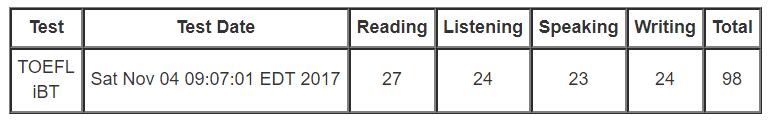
\includegraphics{TOEFL.PNG}
\end{figure}


\newpage
\par{\centering\Large \hypertarget{grds}{B.S. in Naval Architecture and Ocean Engineering}\par}\large{\centering Grades\par}\normalsize
\begin{center}
\begin{tabular}{lcc}
\multicolumn{1}{c}{\textsc{Courses}}&\textsc{Grade}&\textsc{Credit}\\ \hline
Calculus I	&66&	6\\
Calculus II	&91&	4\\
Linear Algebra	&90&	3\\
Mathematical Methods in Physics	&82&	3\\
Probability and Statistics	&83&	3\\
Physics I	&94& 4\\
Physics II	&91&	4\\
Physics Lab. I	&86&	1\\
Physics Lab. II &85&    1\\
Chemistry	&90&	2\\
Chemistry Lab   &88&    1\\
Introduction to Electronics	&95&	3\\ 
Thinking and Approach of Programming	&86&	3\\
Circuit Theory	&72&	3\\
Introduction to Engineering	&100&	3\\
Theoretical Mechanics	&73&	4\\ 
Engineering Drafting I	&86&	2\\
Materials Mechanics	&85&	4\\ \\
		
Ship Vibrations	&82&    2\\
Introduction to Marine Hydrodynamics	&85&    4\\
Shipping Trade and Marketing    &86&    2\\
Ship Construction and Drawing   &88&    3\\
Introduction to Naval Architecture and Ocean Engineering &88&   2\\
Principles of Naval Architecture(I-Statics and Resitance)   &89& 3\\
Marine Structural Mechanics &89&    4\\
Theory of High Perfermance Ships    &92&  2\\
Innovative Experiment of Marine Engineering &93& 3\\ \\
		& Total&79\\\cline{2-3}
&\textsc{Major Gpa}&\textbf{85.68}\\

Introduction to Biology &74&    3\\
Systems Engineering     &77&    2\\
Ocean Engineering Environment   &74&    2\\
Appreciation of English Classics    &85&    2\\
Economy and Law &86&    2\\
Public Speaking in English &87& 2\\
Economics   &88&    2\\
Career Development and Planning &90&    2\\
Selected Readings from Zhuangzi and Laozi   &91&    3\\
Political Comments  &92&    2\\
University English I &71&   3\\
University English II &73&  3\\
University English III &82& 3\\
Physical Education I    &88& 1\\
Physical Education II   &94&    1\\
Physical Education III  &91&    1\\
Physical Education IV   &98&    1\\
Sport Culture           &80&    1\\
\end{tabular}
\end{center}
\begin{center}
\begin{tabular}{lcc}
Military Theory         &87&    1\\
Modern Chinese History  &85&    2\\
Cultivation of Ethics and Fundamentals of Law   &87&    3\\
Basic Theory of Marxism     &82&    3\\
Introduction to Mao Zedong's Thoughts and Theoretical  & &\\
\quad System of Socialism with Chinese Characteristics    &94&    6\\\\

Circumstance and Policy I   &90&     1\\
Circumstance and Policy II  &85&    1\\
Circumstance and Policy III &90&     1\\
Circumstance and Policy IV  &90&     1\\
Engineering Practice        &85&    6\\
Undergraduate Innovation Program of SJTU(IPP14043)  &80&    3\\
The World of Plato  &95&    3\\

		& Total&145\\\cline{2-3}
&\textsc{Overall GPA}&\textbf{85.34}\\
Military Training       &P& 3\\
Lectures on Engineering Frontiers   &P& 1\\
General Education Practice  &P&     2\\
\end{tabular}
\end{center}


\bigskip
\hrule
\bigskip
\par{\centering\Large \hypertarget{grds_usc}{B.S. in Mathematics}\par}\large{\centering Grades\par}\normalsize

\begin{center}
\begin{tabular}{lcc}
\multicolumn{1}{c}{\textsc{Exam}}&\textsc{Grade}&\textsc{Credit}\\ \hline
Mathematical Analysis I &96&    3\\
Mathematical Analysis II &85&   3\\
Numerical Analysis      &80&    3\\
Ordinary Differential Equations &83&    3\\

& &\\\cline{2-3}
 &\textsc{Gpa}&\textbf{86}
\end{tabular}
\end{center}
%\newpage
%\hypertarget{gmat}{\textsc{Gmat}\setmainfont{LMRoman10 Regular}\textregistered\setmainfont[SmallCapsFont=Fontin-SmallCaps]{Fontin-Regular}}

%\XeTeXpdffile ''GMAT.pdf'' page 1 scaled 800

\end{document}
